\section{Main Results}

\subsection{Settings}

\subsubsection{Bandit}

We first analyze the standard bandit setting, i.e., $n = 1$ , and then generalize the results to many state dependent bandits setting. For simplicity, assume the reward $\rvr \in \sR^h$ is a deterministic vector. Using concentration the results can be generalized to random reward vectors, therefore recovering the stochastic bandit setting. Also we assume $r_k \in [0, 1]$, $\forall k \in [h]$.

In this setting, we use the NN policy to pull one arm $A_t \in [h]$ in each time step $t$, then observe the reward $r_{A_t}$. The policy net then uses the reward to update its weight vectors, using policy gradient method. After such $T$ steps, we are concerned with the regret,
\begin{equation*}
    \ell \triangleq \regret(\rvpi) \triangleq \r^{\max} \cdot T - \sum\limits_{t=0}^{T-1}{ \rvpi(t)^\top \rvr } = \sum\limits_{t=0}^{T-1}{ \rvpi(t)^\top \rvtilder }
\end{equation*}

\subsubsection{Episodic MDP}

In the Episodic MDP setting, in each time step, we use NN policy to take one action $A_t$, then observe a reward $R_{t+1}$ and next state $S_{t+1}$. After such $H$ steps, there is an ending state, and this trajectory terminates. Since we use policy gradient method (no value learning method here), the policy updates its weights using the cumulative reward collected from each trajectory. 


\subsection{Policy Gradient Method}

\begin{algorithm}[h]
   \caption{Policy Gradient Method Mixed with Uniform Exploration}
\label{alg:policy_gradient_uniform_exploration}
\begin{algorithmic}
   \STATE {\bfseries Input:} state feature vectors $\rvs_i$
   \STATE Initialize $\rvw_r \sim \gN\left( 0, \sigma \cdot \rmI \right)$, $\forall r \in [m]$, $\rva_k \sim \gN(0, \rmI)$, $\forall k \in [h]$.
   \FOR{$t=0$ {\bfseries to} $T-1$}
   \IF{$t < \sqrt{T}$}
   \STATE Uniformly randomly take action $A_{i,t}$. 
   \STATE Observe reward and next state.
   \ELSE
   \STATE Take action $A_{i,t} \sim \rvpi_{i}\left(\cdot \middle| S_{i,t} \right)$. 
   \ENDIF
   \STATE $\rvw_r(t+1) = \rvw_r(t) - \eta \cdot \frac{d\ell}{d \rvw_r(t)}$, $\forall r \in [m]$.
   \ENDFOR
\end{algorithmic}
\end{algorithm}

The objective of our analysis is the policy gradient method, mixed with uniform exploration, as shown in shown in \cref{alg:policy_gradient_uniform_exploration}. The reason why we need exploration will be explained later on, and technically it seems cannot be eliminated.

The policy gradient method works as follows. After initialization, the policy net $\rvpi$ will be updated using policy gradient calculated from collected reward. In the first $\sqrt{T}$ steps, actions are selected up to an uniform distribution over all actions. After that the NN policy $\rvpi$ is used to select actions.

\subsection{Main Results}
\label{subsec:main_results}

The first main result of the bandit setting is summarized in \cref{thm:main_result_1}.

\begin{thm}
\label{thm:main_result_1}
    Assume $m \in \tilde{\Theta}\left( \frac{n^{10}}{c^4 \delta^4 \varepsilon^2} \right)$, $\eta \in \Theta\left( \frac{c^2 \delta^2}{16 n^4 h m \left( \log{\left(4m\right)} \right)^2} \right)$, after $t \in O\left( \frac{n^4}{\eta m c^2 \delta^2 \varepsilon} \right)$ iterations, $\rvpi_i\left( \rmW(t) \right)^\top \rvtilder_i \le \varepsilon$, and the regret $\sum\limits_{t=1}^{T}{ \rvpi_i\left( \rmW(t) \right)^\top \rvtilder_i } \le  \frac{8 n^4 \sqrt{h}}{c^2 \delta^2} \cdot \tilde{O}\left( \sqrt{T} \right)$.
\end{thm}
\begin{proof}
    By \cref{lem:gradient_upper_bound}, let $\tau = \frac{\sigma}{n}$, there is $\Omega\left( m \right)$ of $\rvw_r(t)$ such that $\left\| \frac{d\ell}{d \rvw_r(t)} \right\|_2 = \left\| \frac{d\tilde{\ell}}{d \rvw_r(t)} \right\|_2$, $\forall t \in O\left( \frac{\sigma}{\eta n \sqrt{\log{m}}} \right)$. Let $\rmW(t+1) = \rmW(t) - \eta \cdot \frac{d \ell}{d \rmW(t)}$, by \cref{lem:semi_smoothness},
\begin{equation*}
\begin{split}
    &\rvpi_i\left( \rmW(t+1) \right)^\top \rvtilder_i \le \rvpi_i\left( \rmW(t) \right)^\top \rvtilder_i - \eta \cdot \left\| \frac{d \ell}{d \rmW(t)} \right\|_F^2 \\
    &\qquad + 4 \sqrt{m \log{\left(4m\right)}} \cdot \rvpi_i\left( \rmW \right)^\top \rvtilder_i \cdot \eta \cdot \left\| \frac{d \ell}{d \rmW(t)} \right\|_F \\
    &\qquad + 4 h m \log{\left(4m\right)} \cdot \eta^2 \left\| \frac{d \ell}{d \rmW(t)} \right\|_F^2 \\
    &\le \rvpi_i\left( \rmW(t) \right)^\top \rvtilder_i - \eta \cdot \sum\limits_{r=1}^{m}{ \left\| \frac{d\ell}{d \rvw_r(t)} \right\|_2^2 } \\
    &\qquad + 4 \sqrt{m \log{\left(4m\right)}} \cdot \rvpi_i\left( \rmW \right)^\top \rvtilder_i \cdot \eta \cdot \sum\limits_{r=1}^{m}{ \left\| \frac{d\ell}{d \rvw_r(t)} \right\|_2 } \\
    &\qquad + 4 h m \log{\left(4m\right)} \cdot \eta^2 \cdot \sum\limits_{r=1}^{m}{ \left\| \frac{d\ell}{d \rvw_r(t)} \right\|_2^2 } \\
    &\le \rvpi_i\left( \rmW(t) \right)^\top \rvtilder_i - \left( \rvpi_i\left( \rmW(t) \right)^\top \rvtilder_i \right)^2 \\
    &\cdot \left[ \frac{\eta m c^2 \delta^2}{n^4} - 8 \eta m \sqrt{m} \log{\left(4m\right)} - 16 \eta^2 h m^2 \left( \log{\left(4m\right)} \right)^2 \right] \\
    &= \rvpi_i\left( \rmW(t) \right)^\top \rvtilder_i - \left( \rvpi_i\left( \rmW(t) \right)^\top \rvtilder_i \right)^2 \cdot \Omega\left( \frac{\eta m c^2 \delta^2}{n^4} \right).
\end{split}
\end{equation*}
Divide $\left( \rvpi_i\left( \rmW(t+1) \right)^\top \rvtilder_i\right) \cdot \left( \rvpi_i\left( \rmW(t) \right)^\top \rvtilder_i \right)$,
\begin{equation*}
\begin{split}
    &\frac{1}{\rvpi_i\left( \rmW(t+1) \right)^\top \rvtilder_i} - \frac{1}{\rvpi_i\left( \rmW(t) \right)^\top \rvtilder_i} \ge \\
    &\frac{\rvpi_i\left( \rmW(t) \right)^\top \rvtilder_i}{\rvpi_i\left( \rmW(t+1) \right)^\top \rvtilder_i} \cdot \Omega\left( \frac{\eta m c^2 \delta^2}{n^4} \right) \ge \Omega\left( \frac{\eta m c^2 \delta^2}{n^4} \right).
\end{split}
\end{equation*}
Sum up the inequality from $0$ to $t$,
\begin{equation*}
\begin{split}
    \frac{1}{\rvpi_i\left( \rmW(t) \right)^\top \rvtilder_i} \ge \Omega\left( \frac{\eta m c^2 \delta^2}{n^4} \right) \cdot t.
\end{split}
\end{equation*}
After $t \in O\left( \frac{n^4}{\eta m c^2 \delta^2 \varepsilon} \right)$ iterations, $\rvpi_i\left( \rmW(t) \right)^\top \rvtilder_i \le \varepsilon$. Let $\frac{n^4}{\eta m c^2 \delta^2 \varepsilon} \le \frac{\sigma}{n \eta \sqrt{\log{m}}} = \frac{1}{n \eta \sqrt{m \log{m}}}$, we have $m \ge \frac{n^{10}}{c^4 \delta^4 \varepsilon^2}\log{\left( \frac{n^{10}}{c^4 \delta^4 \varepsilon^2} \right)}$. Moreover,
\begin{equation*}
\begin{split}
    \sum\limits_{t=1}^{T}{ \rvpi_i\left( \rmW(t) \right)^\top \rvtilder_i } &\le t \cdot 1 + \left(T - t\right) \cdot \varepsilon \\
    &\le t + \frac{n^4}{\eta m c^2 \delta^2} \cdot \frac{T}{t} \\
    &\le \frac{2 n^2}{c \delta} \cdot \frac{1}{\sqrt{\eta m}} \cdot \sqrt{T} \\
    &\le \frac{8 n^4 \sqrt{h}}{c^2 \delta^2} \cdot \log{\left(4m\right)} \cdot \sqrt{T} \\
    &\le \frac{8 n^4 \sqrt{h}}{c^2 \delta^2} \cdot \tilde{O}\left(\sqrt{T}\right). \qedhere
\end{split}
\end{equation*}
\end{proof}

\section{Theoretical Analysis}

We present more detailed analysis than \cref{subsec:main_results}. We first show the bandit case. Note that in the proof of \cref{thm:main_result_1}, the $T$ steps are divided into two parts. In the first $\sqrt{T}$ exploration phase, we uniformly sample actions, and use collected rewards to make the expected regret of NN policy converge to smaller than $\varepsilon$. And in the second commit phase, we use NN policy to play, and because of the expected reward is small, we have the gradient norm lower bounded by positive constant times regret, so the NN policy will keep improving itself. Therefore our analysis will also be partitioned into two parts.

\subsection{Exploring Phase}

In the exploring phase, we uniformly sample actions and rewards to update NN policy. The convergence of policy regret mainly relies on the following ``smoothness" like property over NN weights.

\begin{lem}
    Given weights $\rmW \triangleq \left[ \rvw_1, \rvw_2, \dots, \rvw_m \right]$, and $\rmW^\prime \triangleq \left[ \rvw_1^\prime, \rvw_2^\prime, \dots, \rvw_m^\prime \right]$. Denote $\rvpi_i\left( \rmW \right)$ and $\rvpi_i\left( \rmW^\prime \right)$ as the neural network policies parameterized by $\rmW$ and $\rmW^\prime$, respectively. $\forall i \in [n]$,
\begin{equation*}
\begin{split}
    &\rvpi_i\left( \rmW^\prime \right)^\top \rvtilder_i \le \rvpi_i\left( \rmW \right)^\top \rvtilder_i + \left\langle \frac{d \rvpi_i\left( \rmW \right)^\top \rvtilder_i }{d\left( \rmW \right)}, \rmW^\prime - \rmW \right\rangle \\
    &\qquad + 4 \sqrt{m \log{\left(4m\right)}} \cdot \rvpi_i\left( \rmW \right)^\top \rvtilder_i \cdot \left\| \rmW^\prime - \rmW \right\|_F \\
    &\qquad + 4 h m \log{\left(4m\right)} \cdot \left\| \rmW^\prime - \rmW \right\|_F^2.
\end{split}
\end{equation*}
\end{lem}

Combining this smoothness condition with other objective properties like convexity one can prove convergence results. However, the policy regret is non-convex function of weights. Therefore we need the recent results in overparameterized NN optimization, i.e., the gradient coupling and gradient (lower) bounds.

\begin{lem}
\label{lem:gradient_coupling}
	Define the pseudo gradient as,
\begin{equation*}
\begin{split}
	\frac{d \tilde{\ell}}{d \rvw_r(t)} &\triangleq \frac{1}{n} \cdot \sum\limits_{i=1}^{n}{ \sum\limits_{k=1}^{h}{ \tilde{r}_{i,k} \cdot \pi_{i,k}(t) \cdot \left( \sum\limits_{k^\prime = 1}^{h}{ a_{k^\prime,r}  \cdot v_{k^\prime,k,i}(t) } \right) } } \\
	&\qquad { { \cdot \sI\left\{ \rvw_r(0)^\top \rvs_i > 0 \right\} \cdot \rvs_i } },
\end{split}
\end{equation*}
where $v_{k^\prime,k,i}(t)$ is defined as,
\begin{equation*}
	v_{k^\prime,k,i}(t) = \begin{cases}
    1 - \pi_{i,k^\prime}(t), & \text{if $k^\prime = k$}, \\
    - \pi_{i,k^\prime}(t), & \text{otherwise}.
  \end{cases}
\end{equation*}
	For any $\tau > 0$, with probability at least $\frac{1}{2} \cdot \left( 1 - \frac{\sqrt{2}n\tau}{\sqrt{\pi}\sigma} \right)$, $\forall t \in O\left(\frac{\tau}{\eta  \sqrt{\log{m}}}\right)$, $\forall r \in [m]$,
\begin{equation}
	\frac{d\ell}{d \rvw_r(t)} = \frac{d \tilde{\ell}}{d \rvw_r(t)}.
\end{equation}
\end{lem}

The true gradient can be calculated as,
\begin{equation*}
\begin{split}
    \frac{d\ell}{d \rvw_r(t)} &= \frac{1}{n} \cdot \sum\limits_{i=1}^{n}{ \sum\limits_{k=1}^{h}{  \tilde{r}_{i,k} \cdot \pi_{i,k}(t) \cdot \left( \sum\limits_{k^\prime = 1}^{h}{ a_{k^\prime,r}  \cdot v_{k^\prime,k,i}(t) } \right) }} \\
    &\qquad  {{ \cdot \sI\left\{ \rvw_r(t)^\top \rvs_i > 0 \right\} \cdot \rvs_i } }.
\end{split}
\end{equation*}

\cref{lem:gradient_coupling} means $\sI\left\{ \rvw_r(t)^\top \rvs_i > 0 \right\} = \sI\left\{ \rvw_r(0)^\top \rvs_i > 0 \right\} $ for bounded time steps $t$ with constant probability, therefore the true gradient can be replaced with the simpler pseudo gradient.

The next lemma 

\subsection{Playing Phase}

Use an unnumbered first-level section heading for the references, and use a
hanging indent style, with the first line of the reference flush against the
left margin and subsequent lines indented by 10 points. The references at the
end of this document give examples for journal articles \cite{Samuel59},
conference publications \cite{langley00}, book chapters \cite{Newell81}, books
\cite{DudaHart2nd}, edited volumes \cite{MachineLearningI}, technical reports
\cite{mitchell80}, and dissertations \cite{kearns89}.


\if0
% In the unusual situation where you want a paper to appear in the
% references without citing it in the main text, use \nocite
\nocite{langley00}
\fi

\if0
\begin{table}[t]
\caption{Classification accuracies for naive Bayes and flexible
Bayes on various data sets.}
\label{sample-table}
\vskip 0.15in
\begin{center}
\begin{small}
\begin{sc}
\begin{tabular}{lcccr}
\toprule
Data set & Naive & Flexible & Better? \\
\midrule
Breast    & 95.9$\pm$ 0.2& 96.7$\pm$ 0.2& $\surd$ \\
Cleveland & 83.3$\pm$ 0.6& 80.0$\pm$ 0.6& $\times$\\
Glass2    & 61.9$\pm$ 1.4& 83.8$\pm$ 0.7& $\surd$ \\
Credit    & 74.8$\pm$ 0.5& 78.3$\pm$ 0.6&         \\
Horse     & 73.3$\pm$ 0.9& 69.7$\pm$ 1.0& $\times$\\
Meta      & 67.1$\pm$ 0.6& 76.5$\pm$ 0.5& $\surd$ \\
Pima      & 75.1$\pm$ 0.6& 73.9$\pm$ 0.5&         \\
Vehicle   & 44.9$\pm$ 0.6& 61.5$\pm$ 0.4& $\surd$ \\
\bottomrule
\end{tabular}
\end{sc}
\end{small}
\end{center}
\vskip -0.1in
\end{table}
\fi

\if0
\begin{figure}[ht]
\vskip 0.2in
\begin{center}
\centerline{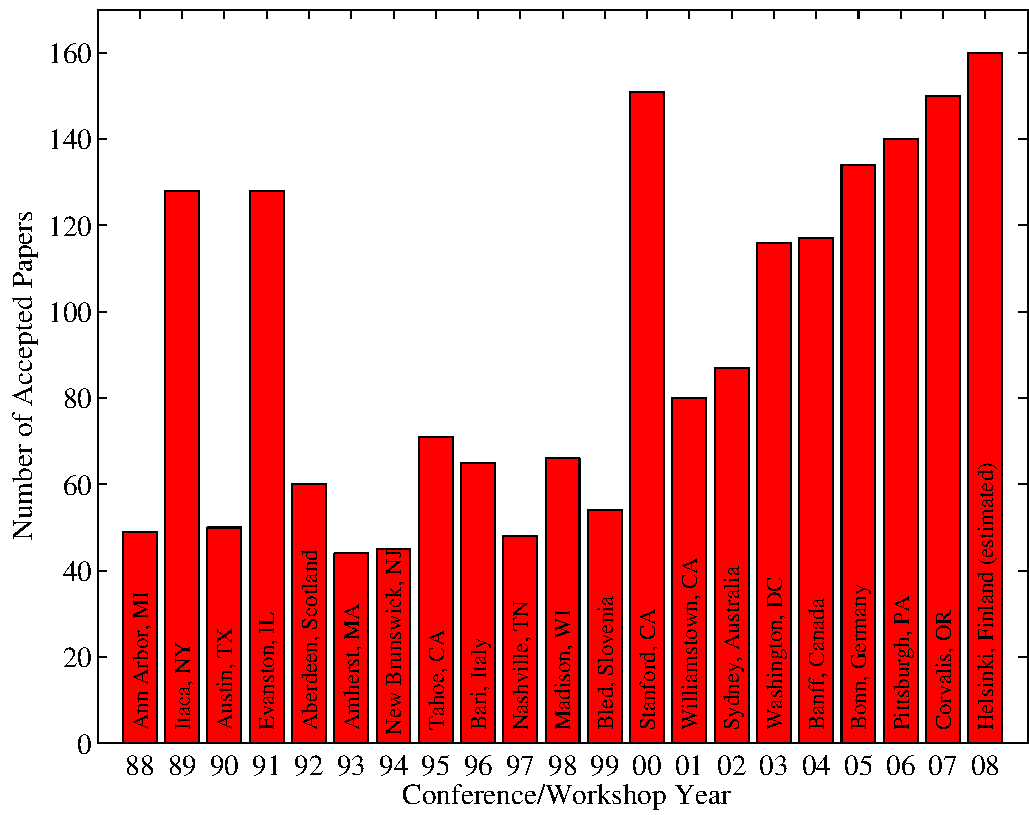
\includegraphics[width=\columnwidth]{icml_numpapers}}
\caption{Historical locations and number of accepted papers for International
Machine Learning Conferences (ICML 1993 -- ICML 2008) and International
Workshops on Machine Learning (ML 1988 -- ML 1992). At the time this figure was
produced, the number of accepted papers for ICML 2008 was unknown and instead
estimated.}
\label{icml-historical}
\end{center}
\vskip -0.2in
\end{figure}
\fi